\section{Updated Opacities}\label{sec:opac}
% Radiative opacity is fundamental to stellar structure, it determines how much
% incident radiation is absorbed or scattered. Moreover, when a media is in
% thermodynamic equilibrium with the radiation field, that is when the temperature
% of the media and that of the radiation field is the same, the opacity may be
% used via Kirchhoff's law to find the emissivity of a material
% \citep{Huebner2014}. Local Thermodynamic Equilibrium (LTE) is a common state to
% find within a star and therefore stellar models have long relied on opacities
% calculated in LTE.
Multiple groups have released high-temperature opacities including the Opacity
Project \citep[OP][]{Seaton1994}, Laurence Livermore National Labs OPAL opacity
tables \citep{Iglesias1996}, and Los Alamos National Labs OPLIB opacity tables
\citep{Colgan2016}. OPAL high-temperature radiative opacity tables in
particular are very widely used by current generation isochrone grids
\citep[e.g. Dartmouth, MIST, \& StarEvol, ][]{Dotter2008,Choi2016,Amard2019}.
However, they are relatively old and therefore do not incorporate the most up to
date understanding of plasma modeling in their code \citep{Colgan2016}

While the two issues given above should  have quite small effects on the CMD as
a whole, the strong theoretical opacity dependence of the Jao Gap raises the
potential for these small effects to measurably shift the gap's location. We
update DSEP to use high temperature opacity tables based on measurements from
Los Alamos national Labs T-1 group \citep[OPLIB,][]{Colgan2016}. The OPLIB
tables use the ATOMIC. ATOMIC \citep{Magee2004,Hakel2006,Fontes2016} is a
modern LTE and non-LTE opacity and plasma modeling code which was used to
generate opacity tables in an attempt to resolve the discrepancy between
helioseismic and solar model predictions of chemical abundances in the sun
\citep{Bahcall2005}. For a detailed breakdown of how the most up-to-date set of
OPLIB tables are generated see \citep{Colgan2013a, Colgan2013b, Colgan2015,
Colgan2016}.

OPLIB tables include monochromatic Rosseland mean opacities --- composed from
bound-bound, bound-free, free-free, and scattering opacities --- for elements
hydrogen through zinc over temperatures 0.5eV to 100 keV and for mass densities
from approximately $10^{-8}$ g cm$^{-3}$ up to approximately $10^{4}$ g
cm$^{-3}$ (though the exact mass density range varies as a function of
temperature). 

When comparing OPAL and OPLIB opacity tables (Figure \ref{fig:opacComp}) we
find OPLIB opacities are systematically lower than OPAL opacities for
temperature above $10^{6}$ K. These lower opacities will decrease the radiative
temperature gradient. Consequently, the radiative layer in a stellar model
evolved using OPLIB opacity tables should be closer into the model core than it
would be in models making use of OPAL tables.

\begin{figure}
	\centering
	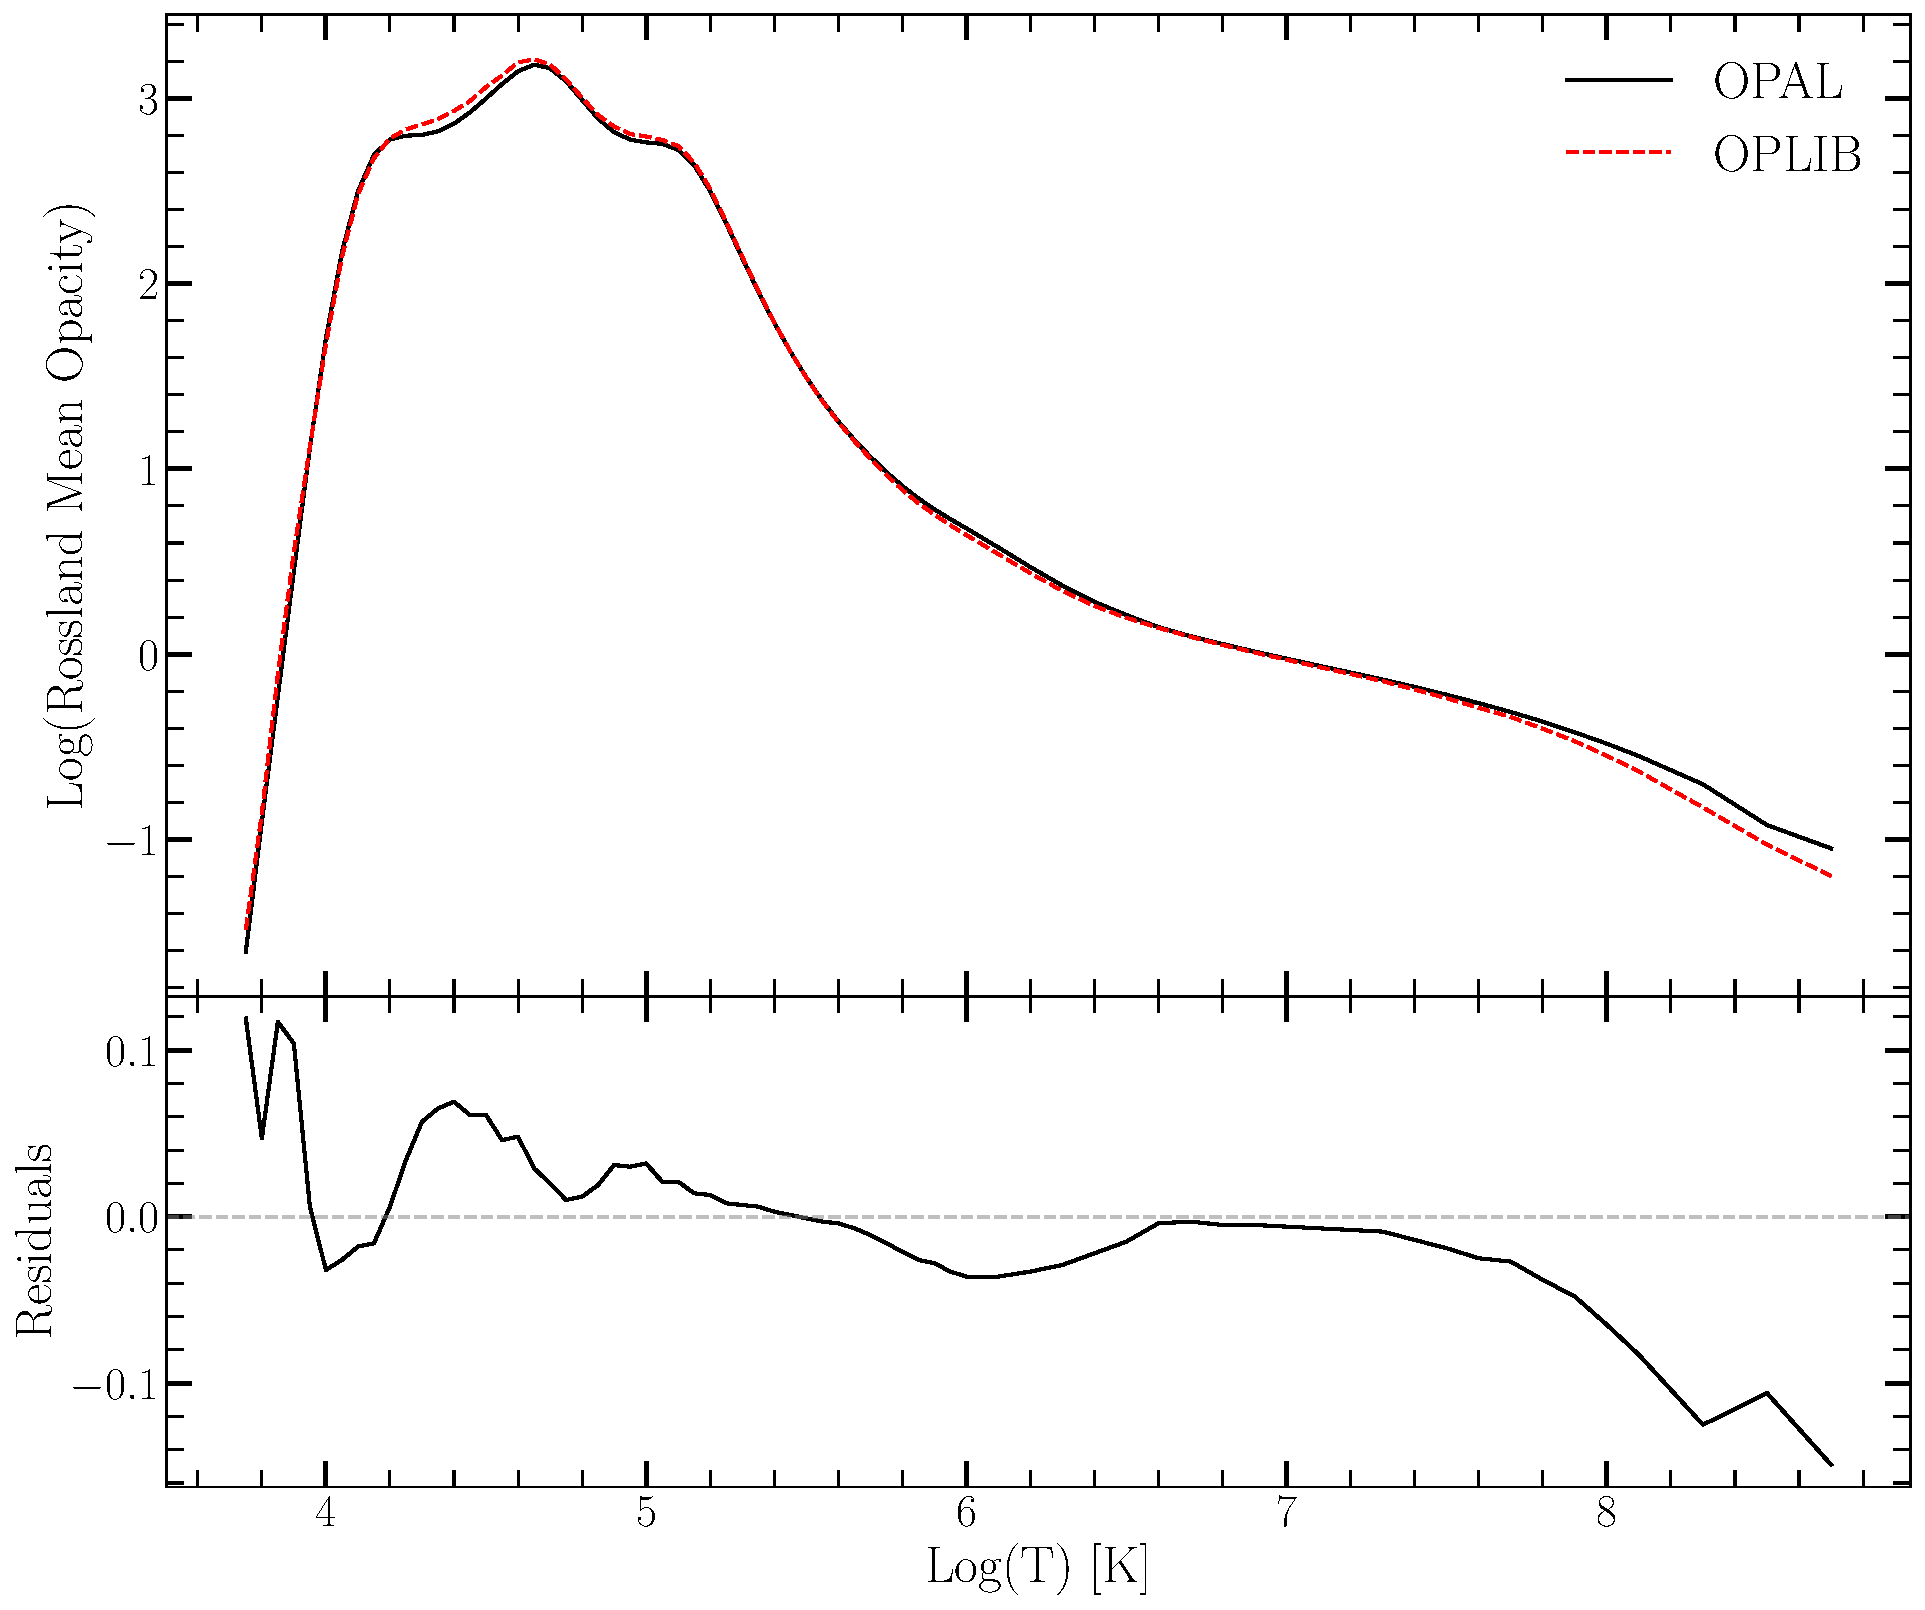
\includegraphics[width=0.45\textwidth]{src/figures/OpacityComparision.pdf}
	\caption{Rosseland mean opacity with the GS98 solar composition for both
	OPAL opacities and OPLIB opacities (top). Residuals between OPLIB opacities
	and OPAL opacities (bottom). These opacities are plotted at $\log _{10}(R)
	= -1.5$, $X=0.7$, and $Z=0.02$. Note how the OPLIB opacities are
	systematically lower than the OPAL opacities for temperatures above $10^6$
	K.}
	\label{fig:opacComp}
\end{figure}

\subsection{Table Querying and Conversion}
The high-temperature opacity tables used by DSEP give Rosseland-mean opacity,
$\kappa_{R}$, along three dimensions: temperature, a density proxy $R$, and
composition. $R$ is defined as

\begin{align} \label{eqn:Req}
	R = \frac{\rho}{T_{6}^{3}}
\end{align}

Where $T_{6} = T\times10^{-6}$ and $\rho$ is the mass density. If $T$ and
$\rho$ are given in cgs then for much of the radius of a star $\log(R)\sim-1.5$
{\color{red}[CITATION]}.  $R$ is used, as opposed to simply tracking opacity
over mass density, because of its small dynamic range when compared to $\rho$ ($\rho\sim
10^{5}$ [g cm$^{-3}$] at the core of an RGB star all the way down to $\sim
10^{-8}$ [g cm$^{-3}$] within the envelope). 

OPLIB tables are queried from a web
interface\footnote{https://aphysics2.lanl.gov/apps/}. In order to generate many
tables easily and quickly we develop a web scraper built with Python's
\texttt{requests} module in addition to the 3rd party \texttt{mechanize} and
\texttt{BeautifulSoup} modules \citep{chandra2015python,
richardson2007beautiful} which can automatically retrieve all the tables needed
to build an opacity table DSEP can make use of. This web scraper submits a user
requested chemical composition (composed of mass fractions for elements from
Hydrogen to Zinc) to the Los Alamos web form, selects 0.0005 keV as the lower
temperature bound and 60 keV as the upper temperature bound, and finally
requests opacity measurements for 100 densities, ranging from $1.77827941\times
10 ^{-15}$ [g cm$^{-3}$] up to $1\times10^{7}$ [g cm$^{-3}$], at each
temperature interval. These correspond to approximately the same temperature
and density range of opacities present in the OPAL opacity tables. For a
detailed discussion of how OPLIB tables are transformed into a format DSEP can
use see Appendix \ref{apx:interp}.

